\documentclass[
	paper=a4,				% set din paper format
	parskip=half,			% vertically separate paragraphs
	bibliography=totoc,     % literature in table of contents
	captions=tableheading,  % table heading
	titlepage=firstiscover, % titlepage is cover
]{scrartcl}

% improve float package
\usepackage{scrhack}
% center overwide objects
\usepackage{adjustbox}

% warn if recompile is necessary
\usepackage[aux]{rerunfilecheck}

% essential math commands
\usepackage{amsmath}
% many math symbols
\usepackage{amssymb}
% extensions for amsmath
\usepackage{mathtools}

% font settings
\usepackage{fontspec} % loads Latin Modern Fonts automatically, alternatives: Libertinus Serif/Sans/Mono

% recalculate page layout after setting differing fonts
\recalctypearea{}

% german language settings
\usepackage[ngerman]{babel}


\usepackage[
	math-style=ISO,		% ┐
 	bold-style=ISO,		% │
	sans-style=italic,	% │ follow iso standard
	nabla=upright,		% │
	partial=upright,	% ┘
	warnings-off={				% ┐
		mathtools-colon,		% │ remove redundant warnings
		mathtools-overbracket,	% ┘
	},
]{unicode-math}

% traditional math fonts
\setmathfont{Latin Modern Math} % alternative: Libertinus Math
\setmathfont[range=\mathbb]{texgyrepagella-math.otf}
% \setmathfont{XITS Math}[range={scr, bfscr}]
% \setmathfont{XITS Math}[range={cal, bfcal}, StylisticSet=1]

% numbers and units num, unit, qty, ang
\usepackage[
	locale=DE,						% german settings
	separate-uncertainty=true,		% always use pm for uncertainties
	per-mode=reciprocal,			% always use negative exponent
%	per-mode=symbol-or-fraction,	% symbol in inline math, fraction in display math
]{siunitx}

% chemical formulas
\usepackage[
	version=4,
	math-greek=default,	% ┐ allow functioning with unicode-math
	text-greek=default,	% ┘
]{mhchem}

% corrected quotation marks
\usepackage[autostyle]{csquotes}

% additional fraction type sfrac to frac, dfrac, tfrac, cfrac
\usepackage{xfrac}

% default placement for floats here, top, bottom
\usepackage{float}
\floatplacement{figure}{htbp}
\floatplacement{table}{htbp}

% control float behaviour
\usepackage[
	section,	% force floats to remain inside section
	below,		% allow placement below section on same page
]{placeins}

% rotate pages to landscape orientation for wide tables
\usepackage{pdflscape}

% improved captions
\usepackage[
	labelfont=bf,			% produce bold label in caption
	font=small,				% reduced fontsize relative to document
	width=0.9\textwidth,	% reduced caption width
]{caption}
% subfigure, subtable, subref
\usepackage{subcaption}

% include graphics
\usepackage{graphicx}

% draw pgf illustrations
\usepackage{tikz}
% draw pgf circuits
\usepackage[european]{circuitikz}

% create tables
\usepackage{booktabs}

% edit enumeration parameters
\usepackage{enumitem}

% improved typeface
\usepackage{microtype}

% bibliography
\usepackage[
	backend=biber,
]{biblatex}
% source database
\addbibresource{lit.bib}
\addbibresource{programme.bib}

% hyperlinks inside document hyperref, href, eqref, ref
\usepackage[
	german,
	unicode,        % allow unicode in pdf attributes
	pdfusetitle,    % title, author, date as pdf attributes
	pdfcreator={},	% ┐ clean up pdf attributes
	pdfproducer={},	% ┘
	hidelinks,		% hide boxes around links
]{hyperref}
% extended bookmarks inside pdf
\usepackage{bookmark}

% separate words with hyphen
\usepackage[shortcuts]{extdash}

% increase bracket size for nesting
\delimitershortfall=-1pt

% input useful macros
% Hammerite, https://tex.stackexchange.com/a/257122

\usepackage{pgfmath, xparse}

\newlength{\MathStrutDepth}
\newlength{\MathStrutHeight}
\settoheight{\MathStrutHeight}{$\mathstrut$}
\settodepth{\MathStrutDepth}{$\mathstrut$}

\newlength{\NumeratorDepth}
\newlength{\DenominatorHeight}
\newlength{\DepthNegativeDifference}
\newlength{\HeightPositiveDifference}
\newlength{\NumeratorBaselineCorrection}
\newlength{\DenominatorBaselineCorrection}

\newlength{\AdditionalEVSFracVerticalSpacing}
\setlength{\AdditionalEVSFracVerticalSpacing}{0.05mm}

% Fraction with equal top-and-bottom vertical spacing around the bar.
% Suited only to simple fractions that do not appear near other fractions.
% When used alongside other fractions, numerator and denominator baselines
% might not be aligned, which might give ugly results.
% Additionally, the default line thickness for overlines and fractions is restored.
\NewDocumentCommand\pfrac{omom}{%
% 		\Umathfractionrule\displaystyle=0.4pt\relax
% 		\Umathoverbarrule\displaystyle=0.4pt\relax
% 		\Umathoverbarvgap\displaystyle=1.4pt\relax
% 		\Umathfractionrule\textstyle=0.4pt\relax
% 		\Umathoverbarrule\textstyle=0.4pt\relax
% 		\Umathoverbarvgap\textstyle=1.4pt\relax
% 		\Umathfractionrule\crampeddisplaystyle=0.4pt\relax
% 		\Umathoverbarrule\crampeddisplaystyle=0.4pt\relax
% 		\Umathoverbarvgap\crampeddisplaystyle=1.4pt\relax
% 		\Umathfractionrule\crampedtextstyle=0.4pt\relax
% 		\Umathoverbarrule\crampedtextstyle=0.4pt\relax
% 		\Umathoverbarvgap\crampedtextstyle=1.4pt\relax
    \IfValueTF{#1}%
              {\settodepth{\NumeratorDepth}{$#1$}}%
              {\settodepth{\NumeratorDepth}{$#2$}}%
    \IfValueTF{#3}%
              {\settoheight{\DenominatorHeight}{$#3$}}%
              {\settoheight{\DenominatorHeight}{$#4$}}%
    \pgfmathsetlength%
        {\DepthNegativeDifference}%
        {\NumeratorDepth - \MathStrutDepth}%
    \pgfmathsetlength%
        {\HeightPositiveDifference}%
        {\MathStrutHeight - \DenominatorHeight}%
    \pgfmathsetlength%
        {\NumeratorBaselineCorrection}%
        {\AdditionalEVSFracVerticalSpacing + \DepthNegativeDifference + \HeightPositiveDifference}%
    \pgfmathsetlength%
        {\DenominatorBaselineCorrection}%
        {-\AdditionalEVSFracVerticalSpacing}%
    \def\Numerator{\raisebox{\NumeratorBaselineCorrection}{$#2$}}%
    \def\Denominator{\raisebox{\DenominatorBaselineCorrection}{$#4$}}%
    \frac{\Numerator}{\Denominator}%
}
 % fraction type with equal v and h spacing pfrac

% tighter dotting in table of contents
\makeatletter
	\renewcommand\@dotsep{2}
	\renewcommand\@pnumwidth{0.75em}
\makeatother

\author{
	Fritz Agildere\\ % Name
	\href{mailto:fritz.agildere@udo.edu}{fritz.agildere@udo.edu} % Email
	\and
	Amelie Strathmann\\ % Name
	\href{mailto:amelie.strathmann@udo.edu}{amelie.strathmann@udo.edu} % Email
}
\publishers{TU Dortmund – Fakultät Physik}


\subject{VERSUCH NUMMER}
\title{TITEL}
\date{
  Durchführung: DATUM
  \hspace{3em}
  Abgabe: DATUM
}

\begin{document}

\maketitle
\thispagestyle{empty}
\tableofcontents
\newpage

\section{Ziel}
\label{sec:Ziel}
% Theorie: Physikalische Grundlagen von Versuch/Messverfahren, Gleichungen ohne Herleitung knapp erklären
\section[Theorie]{Theorie \textnormal{\cite{paramagnet}}}
\label{sec:theorie}

\subsection{Magnetismus und Materie}

Der im Vakuum geltende Zusammenhang zwischen magnetischer Flussdichte $\symbf B$ und magnetischer Feldstärke $\symbf H$
\begin{equation*}
	\symbf B = \mu_0 \symbf H
	\label{eqn:vakuum}
\end{equation*}
muss unter Anwesenheit von Materie um die Magnetisierung $\symbf M$ zu
\begin{equation*}
	\symbf B = \mu_0 \symbf H + \symbf M
	\label{eqn:materie}
\end{equation*}
ergänzt werden. Dabei beschreibt $\mu_0$ die magnetische Feldkonstante. Verantwortlich für das Auftreten von $\symbf M$
sind atomare magnetische Momente im betrachteten Material. Daher lässt sich die Magnetisierung mit dem mittleren
magnetischen Moment $\bar{\symbf \mu}$ und der Anzahl der Momente pro Volumen $N$ als
\begin{equation}
	\symbf M = N \mu_0 \, \bar{\symbf \mu}
	\label{eqn:magnet_moment}
\end{equation}
ausdrücken. Ihre Abhängigkeit zu $\symbf H$ wird über
\begin{equation}
	\symbf M = \mu_0 \, \chi \symbf H
	\label{eqn:magnet_feld}
\end{equation}
formuliert. Der Faktor $\chi$ heißt magnetische Suszeptibilität und weist selbst komplexe Beziehungen zur Feldstärke
$\symbf H$ und Temperatur $T$ auf.

\subsubsection{Diamagnetismus}

Durch die Induktion magnetischer Momente beim Einwirken äußerer Magnetfelder tritt in allen Atomen das Phänomen des
Diamagnetismus auf. Das induzierte Feld ist dem ursächlichen dabei entgegengesetzt und schwächt so dessen Einfluss ab.
Für die Suszeptibilität muss dann $\chi < 0 $ gelten. Ideale Diamagneten werden durch Supraleiter realisiert, welche
$\chi = -1$ erreichen und das Magnetfeld in ihrem Inneren vollständig verdrängen.

\subsubsection{Paramagnetismus}

Anders als der Diamagnetismus ist der Paramagnetismus keine universelle Eigenschaft der Materie, sondern lässt sich nur
bei Atomen, Ionen und Molekülen beobachten, deren Gesamtdrehimpuls nicht verschwindet. Bei Abwesenheit eines äußeren
Feldes sind die an den Drehimpuls gekoppelten magnetischen Momente durch thermische Bewegung zufällig orientiert, sodass
keine mittlere Magnetisierung existiert. Wird jedoch ein Magnetfeld angelegt, richten sich die Momente parallel dazu aus,
sodass dessen Wirkung verstärkt wird. Die Suszeptibilität erfüllt dann $\chi > 0$ und ist aufgrund des Störeinflusses der
thermischen Bewegung temperaturabhängig. Anhand dieses Modells kann $\chi$ nun berechnet werden.

\subsection{Paramagnetische Suszeptibilität} 

Der atomare Gesamtdrehimpuls $\symbf J$ setzt sich aus Bahndrehimpuls der Elektronenhülle und Eigendrehimpuls der
Elektronen, dem Spin, zusammen. Für den Paramagnetismus kann der Beitrag des zusätzlich auftretenden Kerndrehimpulses
vernachlässigt werden. Solange das äußere Magnetfeld nicht zu stark ist, wird von LS-Kopplung mit
\begin{equation*}
	\symbf J = \symbf L + \symbf S
	\label{eqn:kopplung}
\end{equation*}
ausgegangen, also der Annahme, dass $\symbf J$ der Vektorsumme von Gesamtbahndrehimpuls~$\symbf L$ und Gesamtspin
$\symbf S$ entspricht. Dabei setzen sich $\symbf L$ und $\symbf S$ nach
\begin{align*}
	\symbf L = \sum_i \symbf l_i && \symbf S = \sum_i \symbf s_i
\end{align*}
aus der jeweiligen Vektorsumme der Einzeldrehimpulse sämtlicher in der Hülle enthaltenen Elektronen zusammen. Anwenden
quantenmechanischer Mittel liefert dann die zugehörigen magnetischen Momente, welche sich auf
\begin{align}
	\symbf \mu_L &= - \frac{\mu_B}{\hbar} \symbf L \label{eqn:mu_L}
	\shortintertext{und}
	\symbf \mu_S &= - g_s \frac{\mu_B}{\hbar} \symbf S \label{eqn:mu_S}
\end{align}
belaufen. Dabei entspricht $\hbar = \frac{h}{2\pi}$ der reduzierten Planck-Konstante, die mit Wirkungsquantum $h$,
Frequenz $\nu$ und Kreisfrequenz $\omega$ die Beziehung $h \nu = \hbar \omega$ erfüllt. Mit der Ladung $e_0$ und
Ruhemasse $m_0$ des Elektrons bezeichnet das Bohrsche Magneton
\begin{equation*}
	\mu_B = \frac{1}{2} \frac{e_0}{m_0} \hbar
	\label{eqn:magneton}
\end{equation*}
das zur Drehimpulseinheit $\hbar$ gehörige magnetische Moment. Ebenso ist mit der negativen Ladung des Elektrons das
negative Vorzeichen in \eqref{eqn:mu_L} und \eqref{eqn:mu_S} erklärt. Der Faktor $g_S$ entspricht dem gyromagnetischen
Verhältnis des freien Elektrons.

Unter Verwendung der Bahndrehimpulsquantenzahl $L$, Spinquantenzahl $S$ und Gesamtdrehimpulsquantenzahl $J$ des Atoms lässt sich
\begin{align}
	| \symbf L | = \sqrt{L(L+1)} \hbar &&
	| \symbf S | = \sqrt{S(S+1)} \hbar &&
	| \symbf J | = \sqrt{J(J+1)} \hbar \label{eqn:abs}
\end{align}
für die Beträge der Drehimpulse schreiben. Aus \eqref{eqn:mu_L} und \eqref{eqn:mu_S} folgt damit weiter
\begin{align}
	| \symbf \mu_L | &= \frac{\mu_B}{\hbar} | \symbf L | = \mu_B \sqrt{L(L+1)} \label{eqn:abs_mu_L}
	\shortintertext{und}
	| \symbf \mu_S | &= g_s \frac{\mu_B}{\hbar} | \symbf S | = g_S \, \mu_B \sqrt{S(S+1)} \label{eqn:abs_mu_S}
\end{align}
für die entsprechenden magnetischen Momente. Bei LS-Kopplung verschwindet die zu $\symbf J$ orthogonale Komponente von $\symbf \mu$,
sodass nur $\symbf \mu_J \parallel \symbf J$ messbar ist. In Abbildung \ref{fig:diagramm} kann dazu der Zusammenhang
\begin{equation}
	| \symbf \mu_J | = | \symbf \mu_S | \cos \alpha + | \symbf \mu_L | \cos \beta
	\label{eqn:abs_mu_J}
\end{equation}
abgelesen werden. Zudem lässt sich nach dem Cosinussatz mittels des Dreiecks $OAB$
\begin{align}
	\cos \alpha = \frac{ | \symbf J |^2 - | \symbf L |^2 + | \symbf S |^2 }{2| \symbf J || \symbf S |} &&
	\cos \beta = \frac{ | \symbf J |^2 + | \symbf L |^2 - | \symbf S |^2 }{2| \symbf J || \symbf S |}
	\label{eqn:cosine}
\end{align}
aus Abbildung \ref{fig:diagramm} herleiten.

\begin{figure}[H]
	\centering
	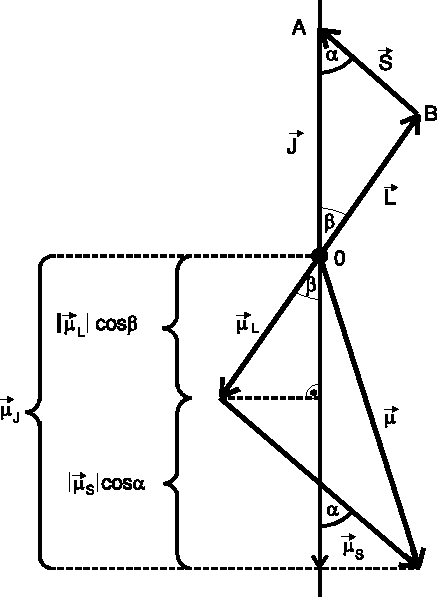
\includegraphics{content/grafik/diagramm.pdf}
	\caption{Vektordiagramm der Drehimpulse einer Elektronenhülle mit den resultierenden magnetischen Momenten.}
	\label{fig:diagramm}
\end{figure}

Einsetzen von \eqref{eqn:abs}, \eqref{eqn:abs_mu_L}, \eqref{eqn:abs_mu_S} und \eqref{eqn:cosine} in die Beziehung
\eqref{eqn:abs_mu_J} liefert nun
\begin{align*}
	| \symbf \mu_J | &= \mu_B \left( g_S \sqrt{S(S+1)} \cos \alpha + \sqrt{L(L+1)} \cos \beta \right) \\
	&= \mu_B \frac{(g_S + 1)J(J+1) + (g_S - 1) \left( S(S+1) - L(L+1) \right) }{2\sqrt{J(J+1)}}
\end{align*}
als Betrag des magnetischen Moments. Anhand der Größe $g_S$ kann mit guter Genauigkeit die Näherung $g_S \approx 2$ ausgenutzt werden,
um über den für das Atom spezifischen Landé-Faktor
\begin{equation*}
	g_J = \frac{3J(J+1) + \left( S(S+1) - L(L+1) \right)}{2J(J+1)}
	\label{eqn:lande}
\end{equation*}
den Ausdruck
\begin{equation}
	| \symbf \mu_J | \approx \mu_B \, g_J \sqrt{J(J+1)}
	\label{eqn:approx_abs_mu_J}
\end{equation}
zusammenzufassen. Ein weiteres quantenmechanisches Phänomen ist die Richtungsquantelung, wonach der Winkel zwischen einem äußeren
Magnetfeld und $\symbf \mu_J$ nicht beliebig ist, sondern nur solche Werte einnimmt, bei denen die Komponente $\mu_{J_z}$ von
$\symbf \mu_J$ in Feldrichtung ein ganzzahliges Vielfaches von $\mu_B g_J$ darstellt. Entsprechend muss
\begin{equation*}
	\mu_{J_z} = - \mu_B \, g_J \, m
	\label{eqn:komponente}
\end{equation*}
gelten, wobei $m \in \symbb{Z}$ die Orientierungsquantenzahl bezeichnet. Da $\mu_{J_z}$ als Komponente von $\symbf \mu_J$ immer
$| \mu_{J_z} | \leq | \symbf \mu_J |$, also laut \eqref{eqn:approx_abs_mu_J} $m \leq \sqrt{J(J+1)}$ erfüllt, führt die Einschränkung
$m \in \{ -J, -J+1, \dotsc, 0, \dotsc, J-1, J \}$ zu dem Schluss, dass genau $2J+1$ Möglichkeiten zur Einstellung des magnetischen
Moments relativ zur äußeren Feldrichtung existieren. Jeder dieser Einstellrichtungen lässt sich eine spezifische potentielle
Energie
\begin{equation*}
	E_m = - \symbf \mu_J \cdot \symbf B = \mu_{J_z} B = \mu_B \, g_J \, m B
	\label{eqn:zeeman}
\end{equation*}
zuordnen. Dieses Auftreten von $2J+1$ Unterenergieniveaus heißt Zeeman-Effekt. Deren Besetzungshäufigkeit folgt mit
\begin{equation*}
	Z(E_m,T) = \exp \! \left( - \pfrac{E_m}{kT \,} \right)
	\label{eqn:boltzmann}
\end{equation*}
einer Boltzmann-Verteilung, Summation über alle Niveaus liefert
\begin{equation*}
	\mu_\text{ges} = \sum_{m = -J}^J -\mu_B \, g_J \, m Z(E,T) = -\mu_B \, g_J
	\sum_{m = -J}^J m \, \exp \! \left( - \frac{\mu_B \, g_J \, mB}{kT \,} \right)
	\label{eqn:mu_ges}
\end{equation*}
für das gesamte magnetische Moment.
\newpage
Nach Division durch die Gesamthäufigkeit aller vorkommenden Orientierungen ergibt sich daraus
\begin{equation}
	\bar{\mu} = - \mu_B \, g_J \, \frac{\displaystyle{\sum_{m = -J}^J m \, \exp \! \left( - \frac{\mu_B \, g_J \, mB}{kT \,} \right)}}
	{\displaystyle{\sum_{m = -J}^J \exp \! \left( - \frac{\mu_B \, g_J \, mB}{kT \,} \right)}}
	\label{eqn:mu_mittel}
\end{equation}
als Betrag des in \eqref{eqn:magnet_moment} geforderten mittleren magnetischen Moments. Der Quotient in Ausdruck~\eqref{eqn:mu_mittel}
wird als Brillouin-Funktion bezeichnet. Bei einer Temperatur im Bereich $T \approx \qty{300}{\kelvin}$ sowie unter Einwirkung von
Flussdichten bis $B \approx \qty{1}{\tesla}$ gilt
\begin{equation*}
	\frac{\mu_B \, g_J \, mB}{kT} \ll 1
	\label{eqn:kleiner}
\end{equation*}
und erlaubt mit der Entwicklung
\begin{equation*}
	\exp \! \left( - \frac{\mu_B \, g_J \, mB}{kT \,} \right) \simeq 1 - \frac{\mu_B \, g_J \, mB}{kT \,}
	\label{eqn:naeherung}
\end{equation*}
das Aufstellen einer Näherungsformel. So ergibt sich
\begin{equation}
	\sum_{m = -J}^J \left( 1 - \frac{\mu_B \, g_J \, mB}{kT \,} \right) =
	2J + 1 - \frac{\mu_B \, g_J \, B}{kT \,} \sum_{m = -J}^J m = 2J + 1
	\label{eqn:nenner}
\end{equation}
für den Nenner der Funktion, der Zähler ist mit
\begin{equation}
	\sum_{m = -J}^J \left( m - \frac{\mu_B \, g_J \, m^2 B}{kT \,} \right) =
	- \frac{\mu_B \, g_J \, B}{kT \,} \sum_{m = -J}^J m^2 =
	- \frac{\mu_B \, g_J \, B}{3kT \,} J(J+1)(2J+1)
	\label{eqn:zaehler}
\end{equation}
gegeben. Einsetzen von \eqref{eqn:mu_mittel}, \eqref{eqn:nenner} und \eqref{eqn:zaehler} in Gleichung \eqref{eqn:magnet_moment}
liefert den Term
\begin{equation*}
	M = N \mu_0 \, \bar{\mu} = N \mu_0 \, \mu_B^2 \, g_J^2 \, \frac{J(J+1)B}{3kT}
	\label{eqn:magnet_betrag}
\end{equation*}
als Betrag der makroskopischen Magnetisierung. Aus der Äquivalenz \eqref{eqn:magnet_feld} folgt dann mit
\begin{equation}
	\chi = \frac{N \mu_0 \, \mu_B^2 \, g_J^2 \, J(J+1)}{3kT}
	\label{eqn:chi_theo}
\end{equation}
die magnetische Suszeptibilität, welche damit dem Zusammenhang
\begin{equation*}
	\chi \sim \pfrac{1}{T\,}
	\label{eqn:curie}
\end{equation*}
gehorcht. Dabei handelt es sich um das Curiesche Gesetz des Paramagnetismus, dessen Gültigkeit
hiermit für ausreichend hohe Temperaturen belegt ist.

\subsubsection{Seltene-Erd-Verbindungen}

Aus der experimentellen Erkenntnis, dass Verbindungen, die Ionen Seltener Erden enthalten, stark paramagnetisch sind, lässt sich
unter Betrachtung von Formel~\eqref{eqn:chi_theo} auf die Existenz großer Drehimpulse in den Elektronenhüllen Seltener-Erd-Atome
schließen. Dabei muss es sich zudem um innere Elektronen handeln, um den Paramagnetismus auch im ionisierten Zustand zu erklären.
Alle Elemente der Seltenen Erden besitzen mit der vollständigen \ce{Xe}-Hülle Elektronen bis zur 5p- sowie zwei weitere in der
6s-Schale. Diese sind in der weiteren Betrachtung jedoch nicht relevant, da sämtliche Spins und Bahndrehimpulse gesättigt sind.
Es entsteht so kein von Null verschiedener Gesamtdrehimpuls. Vielmehr sind dafür die tiefer befindlichen 4f-Elektronen
verantwortlich, deren Anordnung den Hundschen Regeln unterliegt:
\begin{enumerate}
	\item Einzelne Spins $\symbf s_i$ sind so kombiniert, dass sie den maximalen mit dem Pauli-Prinzip vereinbaren Gesamtspin
			$\symbf S = \sum_i \symbf s_i$ erreichen, sich also möglichst parallel ausrichten. Nach dem Pauli-Prinzip dürfen
			zwei Elektronen nie in all ihren Quantenzahlen übereinstimmen.
	\item Individuelle Bahndrehimpulse $\symbf l_i$ setzen sich so zusammen, dass immer der maximale Gesamtbahndrehimpuls
			$\symbf L = \sum_i \symbf l_i$ auftritt, welcher sowohl mit dem Pauli-Prinzip als auch der 1. Hundschen Regel verträglich ist.
	\item Ist die Schale weniger als halbvoll, tritt ein Gesamtdrehimpuls $\symbf J = \symbf L - \symbf S$ auf. Ist sie mehr als zur
			Hälfte gefüllt, so ist $\symbf J = \symbf L + \symbf S$ gegeben. Sind genau halb so viele Elektronen wie maximal
			möglich vorhanden, folgt $\symbf L = 0$ aus der 2. Hundschen Regel, sodass immer $J = S$ gilt.
\end{enumerate}
Basierend auf der gegenseitigen elektrostatischen Abstoßung der Hüllenelektronen finden die Hundschen Regeln im Folgenden zur
Berechnung der magnetischen Suszeptibilität Anwendung, indem aus ihnen Gesamtdrehimpuls $J$ und Landé-Faktor $g_J$ ermittelt werden.
Speziell im Bezug auf die zu betrachtende 4f-Schale gelten einige Einschränkungen. Als f-Schale ist jeder einzelne Bahndrehimpuls
mit $l_i \leq 3$ beschränkt. Daraus folgt weiter eine vollständige Belegung mit einer maximalen Anzahl von 14 Elektronen.

\subsection{Messverfahren}

\subsubsection{Apparatur zur Induktivitätsmessung}

Die Induktivität einer langen Zylinderspule mit Windungszahl $n$, Querschnittsfläche $F$ und Länge $l$ wird über
\begin{equation}
	L = \mu_0 \pfrac{n^2}{\! l} F
	\label{eqn:spule_vak}
\end{equation}
beschrieben. Ist ihr Inneres gänzlich mit Materie gefüllt, gilt
\begin{equation*}
	L_{\widehat{M}} = \mu \, \mu_0 \pfrac{n^2}{\! l} F
	\label{eqn:spule_mat}
\end{equation*}
mit der Permeabilitätszahl $\mu$ als materialspezifischer Skalierungsfaktor.
\enlargethispage*{\baselineskip}
\newpage
Für einen Probenquerschnitt $Q < F$ muss eine Korrektur
\begin{equation*}
	L_M = \mu_0 \pfrac{n^2}{\! l} F + (\mu - 1) \mu_0 \pfrac{n^2}{\! l} Q =
	\mu_0 \pfrac{n^2}{\! l} F + \chi \mu_0 \pfrac{n^2}{\! l} Q = L + \increment L
	\label{eqn:spule_real}
\end{equation*}
vorgenommen werden. Hierbei wird die Induktivitätsänderung
\begin{equation}
	\increment L = \chi \mu_0 \pfrac{n^2}{\! l} Q
	\label{eqn:diff_real}
\end{equation}
eingeführt. Diese fällt im Allgemeinen sehr gering aus, sodass es einer präzisen Messung bedarf. Diesem Zweck dient die in
Abbildung \ref{fig:schaltung} dargestellte Brückenschaltung.

\begin{figure}[H]
	\centering
	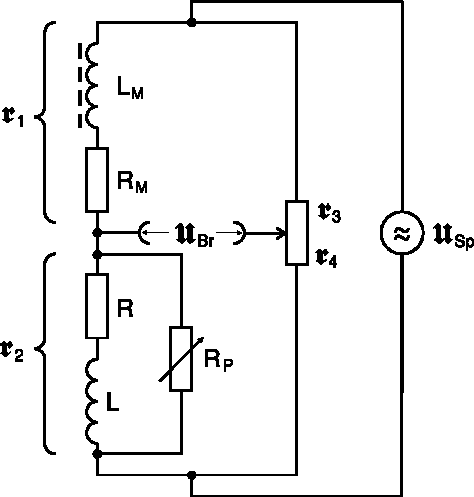
\includegraphics{content/grafik/schaltung.pdf}
	\caption{Brückenschaltung zur präzisen Suszeptibilitätsmessung.}
	\label{fig:schaltung}
\end{figure}

Brückenspannung $\symbffrak U_\text{Br}$ und Speisespannung $\symbffrak U_\text{Sp}$ sind dabei über die Relation
\begin{equation}
	\symbffrak{ U_\text{Br} = \frac{r_4 r_1 - r_3 r_2}{(r_1 + r_2)(r_3 + r_4)} \, U_\text{Sp} }
	\label{eqn:bruecke_gen}
\end{equation}
miteinander verknüpft \cite{brücke}. Dazu lassen sich die komplexen Impedanzen
\begin{align*}
	\symbffrak r_1 = R_M + \symbffrak i \, \omega L_M &&
	\pfrac{1}{\symbffrak r_2} = \pfrac{1}{R_P} + \pfrac{1}{R + \symbffrak i \, \omega L} &&
	\symbffrak r_3 = R_3 && \symbffrak r_4 = R_4
\end{align*}
mit der imaginären Einheit $\symbffrak i$ aufstellen, mit $\omega$ ist die angelegte Spannungsfrequenz bezeichnet.
Um kleinste Unterschiede zwischen den Verlustwiderständen $R$ und $R_M$ der beiden idealerweise identischen Spulen
zu kompensieren, wird der Regelwiderstand $R_P$ verbaut. Für diesen kann $R_P \gg R, \omega L$ angenommen werden, sodass
$\symbffrak r_2 \approx R + \symbffrak i \, \omega L$ gilt.

Aus \eqref{eqn:bruecke_gen} folgt, dass die Abgleichbedingung der Schaltung
\begin{equation}
	\symbffrak r_1 R_4 = \symbffrak r_2 R_3
	\label{eqn:abgleich_ohne}
\end{equation}
ohne Probe für $R_3 \approx R_4$ erfüllt ist. Mit eingebauter Probe wird bei
\begin{equation*}
	R'_3 = R_3 + \increment R
	\label{eqn:R_3}
\end{equation*}
ein neuer Abgleichpunkt gefunden, wegen $R_3 + R_4 = R'_3 + R'_4 = \text{const}$ folgt
\begin{equation*}
	R'_4 = R_4 - \increment R \approx R_3 - \increment R
	\label{eqn:R_4}
\end{equation*}
als Resultat der Implementierung von $R_3$ und $R_4$ als Potentiometer. Durch Einsetzen der neuen Impedanzen folgt aus
\eqref{eqn:abgleich_ohne} die Gleichung
\begin{equation}
	(R_M + \symbffrak i \, \omega L_M)(R_3 - \increment R) = (R + \symbffrak i \, \omega L)(R_3 + \increment R)
	\label{eqn:abgleich_mit}
\end{equation}
als Abgleichbedingung mit durch die Probe veränderter Induktivität. Ihr Imaginärteil lässt sich zu
\begin{equation*}
	\increment R = \frac{R_3 (L_M - L)}{L_M + L}
	\label{eqn:R_delta_1}
\end{equation*}
umformulieren. Einsetzen von $L_M = L + \increment L$ mit der Annahme $\increment L \ll L$ liefert
\begin{equation*}
	\increment R = \frac{R_3 (\increment L)}{2L + \increment L} \approx \frac{R_3 (\increment L)}{2L} 
	\label{eqn:R_delta_2}
\end{equation*}
und weiter mit \eqref{eqn:spule_vak} sowie \eqref{eqn:diff_real} die Formel
\begin{equation*}
	\increment R = \chi \frac{R_3}{2} \frac{Q}{\! F} 
	\label{eqn:R_delta_3}
\end{equation*}
für die notwendige Widerstandsänderung, aus der sich nun
\begin{equation}
	\chi =  2 \pfrac{\increment R}{R_3} \pfrac{F}{Q} 
	\label{eqn:chi_exp}
\end{equation}
zur experimentellen Bestimmung der magnetischen Suszeptibilität ergibt.


\subsubsection{Unterdrückung von Störspannungen}

Die Brückenspannung $\symbffrak U_\text{Br}$ fällt bei der Messung so gering aus, dass sie fast völlig durch das unvermeidbar
auftretende Störrauschen verdeckt wird. Da es sich jedoch um eine monofrequente Signalspannung handelt, ist ein digitaler
Filter durch Sperren aller von der Signalfrequenz $\nu$ verschiedenen Frequenzen in der Lage, die Hintergrundspannungen
zu kompensieren. Ein solches Gerät wird annähernd durch einen Selektivverstärker realisiert, der im wesentlichen aus einem
Bandpass mit Durchlassfrequenz $\nu_0$ besteht. In Abbildung~\ref{fig:kurve} ist ein exemplarischer Verlauf der Ausgangs-
zur Eingangsspannung dargestellt.

\begin{figure}[H]
	\centering
	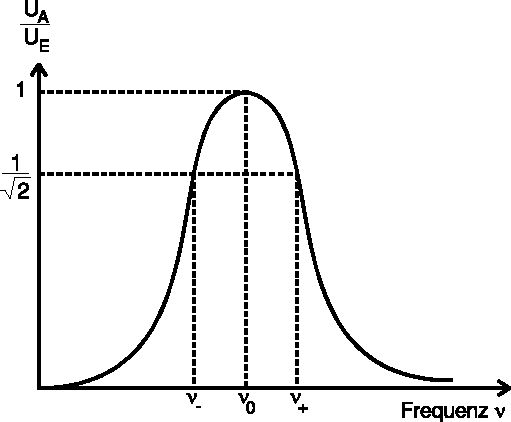
\includegraphics{content/grafik/kurve.pdf}
	\caption{Filterkurve zu Güte und Funktion eines Selektivverstärkers.}
	\label{fig:kurve}
\end{figure}

Es ist zu erkennen, dass für $\nu = \nu_0$ im angrenzenden Frequenzbereich nicht alle Störspannungen unterdrückt sind. Ein Maß für
die Breite dieser Region ist durch die Güte
\begin{equation*}
	Q = \frac{\nu_0}{\nu_+ - \nu_-}
	\label{eqn:gut}
\end{equation*}
gegeben. Das Intervall $\mathopen[ \nu_-, \nu_+ \mathclose]$ enthält hier solche Frequenzen, die
$\sqrt{2} \, U_{\! A} \geq U_E$ erfüllen.

% Vorbereitung: Vorbereitungsaufgaben bearbeiten
% Versuchsaufbau: Verwendete Apparatur, Beschreibung Funktionsweise/Nutzen mit Skizze/Foto
\section{Durchführung}
\label{sec:durchführung}

Zur Vorbereitung können die Schallgeschwindigkeiten von Acryl $c_\text{Acryl} = \qty{2700}{\meter\per\second}$ \cite{doppler}
sowie von destilliertem Wasser und Luft mit $c_\text{Wasser} = \qty{1497}{\meter\per\second}$ und
$c_\text{Luft} = \qty{346}{\meter\per\second}$~\cite{lid_chem_phy} bei einer Temperatur von $\qty{25}{\celsius}$ angegeben werden.
Wegen $\lambda = c / \nu$ und $T = 1 / \nu$ lauten Wellenlänge und Periode in Acryl bei Frequenzen von $\qty{1}{\mega\hertz}$,
$\qty{2}{\mega\hertz}$ und $\qty{4}{\mega\hertz}$ jeweils:

\begin{table}[H]
	\centering
	\begin{tabular}{S[table-format=1.0] S[table-format=1.3] S[table-format=1.2]}
		\toprule
		{$\nu \mathbin{/} \unit{\mega\hertz}$} &
		{$\lambda \mathbin{/} \unit{\milli\meter}$} &
		{$T \mathbin{/} \unit{\micro\second}$} \\
		\midrule
		1 & 2.700 & 1.00 \\
		2 & 1.350 & 0.50 \\
		4 & 0.675 & 0.25 \\
		\bottomrule
	\end{tabular}
\end{table}

\section{Fehlerrechnung}
\label{sec:Fehlerrechnung}

% Messwerte: Alle gemessenen Größen tabellarisch darstellen
% Auswertung: Berechnung geforderter Ergebnisse mit Schritten/Fehlerformeln/Erläuterung/Grafik (Programme)
\section{Auswertung}
\label{sec:auswertung}

\subsection{Fehlerrechnung}
\label{sec:Fehlerrechnung}
Die Fehlerrechnung, für die Bestimmung der Messunsicherheiten, wird mit Uncertainties \cite{uncertainties} gemacht.
Die Formel der Gauß Fehlerfortpflanzung ist gegeben durch
\begin{equation}
    \Delta f=\sqrt{\sum_{i=1}^N\left(\frac{\partial f}{\partial x_i}\right)^2 \cdot\left(\Delta x_i\right)^2}.
    \label{eqn:gauss}
\end{equation}
Für den Mittelwert gilt 
\begin{equation}
    \bar{x} = \frac{1}{N}\sum\limits_{i = 1}^N x_i .
    \label{eqn:mittelwert}
\end{equation}
Der Fehler des Mittelwertes ist gegeben durch 
\begin{equation}
    \Delta \bar{x}=\frac{1}{\sqrt{N}} \sqrt{\frac{1}{N-1} \sum_{i=1}^N\left(x_i-\bar{x}\right)^2}.
    \label{eqn:mittelwertfehler}
\end{equation}

\subsection{Vermessung des Acrylblocks mit einer Schieblehre}
\label{Vermessung des Acrylblocks mit einer Schieblehre}

Der gegeben Acrylblock und dessen Bohrungen wurde wie in \autoref{fig:mess} dargestellt, vermessen.
Der Block ist $\SI{80.4}{\milli\meter}$ breit, $\SI{150.3}{\milli\meter}$ lang und $\SI{40.3}{\milli\meter}$ tief.
Für die Abstände $a_k$ und $b_k$ und den Durchmesser $d$ der jeweiligen Bohrungen wurde ein Ablesefehler von $\SI{0.05}{\milli\meter}$
angenommen.
\begin{figure}[H]
    \centering
    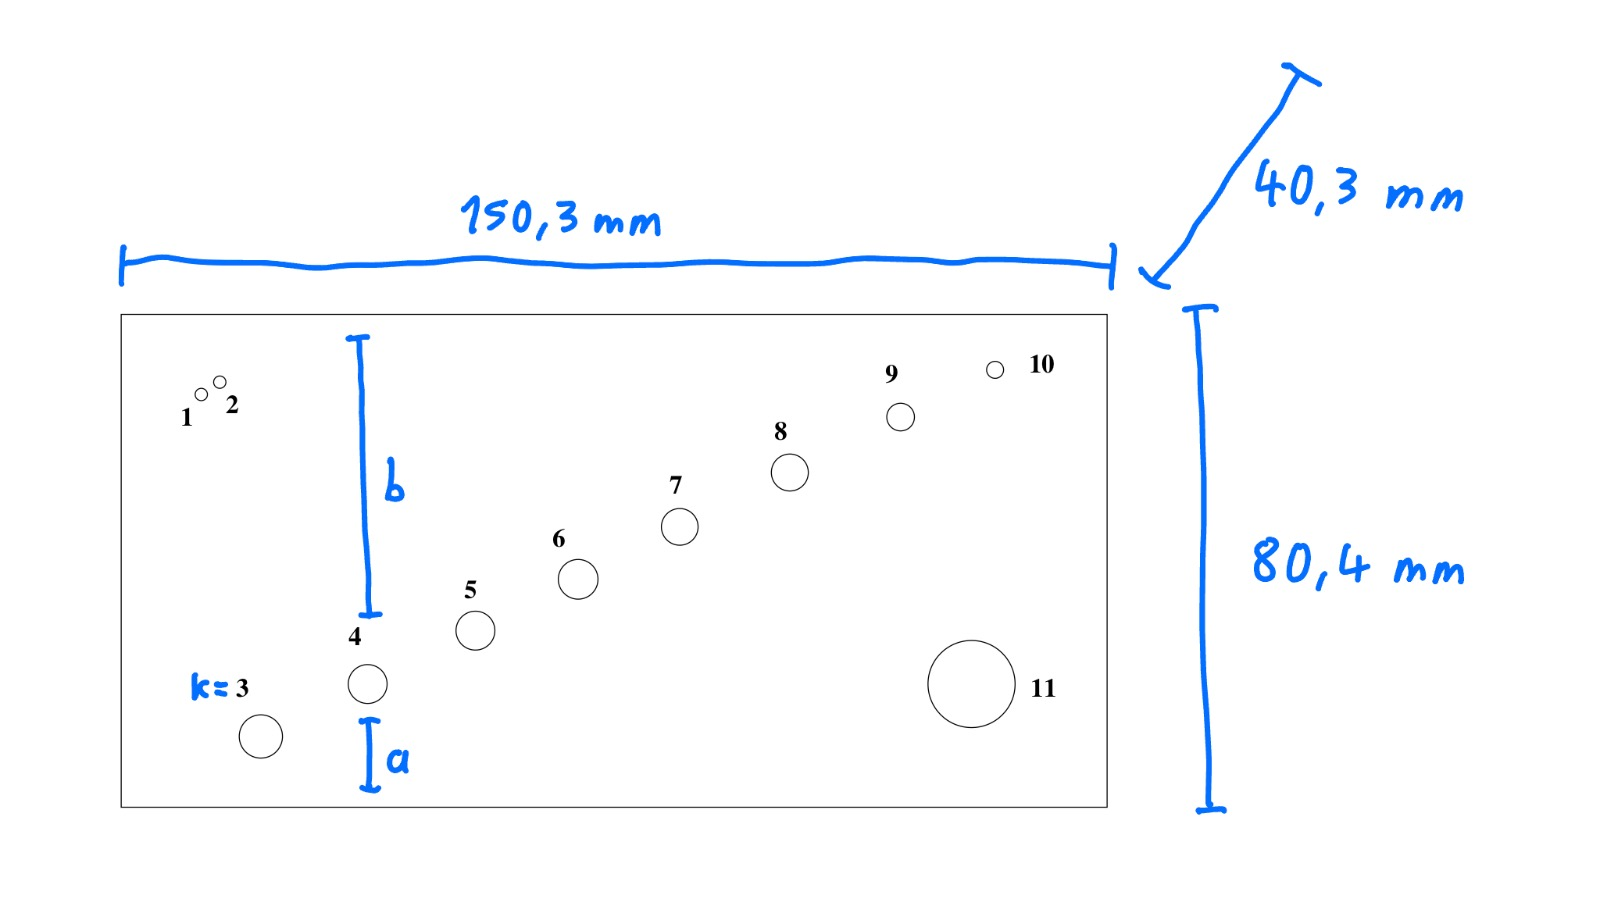
\includegraphics[width=0.9\linewidth]{content/grafik/abmessung.jpg}
	\captionsetup{width=0.765\linewidth}
	\caption{Acrylblock mit Bohrungen und Maßen. \cite{scan}}
    \label{fig:mess}
\end{figure}

Die Messdaten der Abstände $a_k$ und $b_k$ sind in \autoref{tab:lab} zu sehen. 
\begin{table}[H]
    \centering
    \caption{Abmessung der Löcher des Acrylblocks.}
    \label{tab:lab}
\begin{tabular}{c c c c}
    \toprule
    Loch & $a_k / \si{\milli\meter}$ & $b_k / \si{\milli\meter}$ & $d / \si{\milli\meter}$\\
    \midrule
    1 &   -  &    -   & 1.45 \\
    2 &   -  &    -   & 1.5 \\
    3 & 13.5 & 61.85 &    6  \\
    4 &21.85 &  54.4 &  4.9  \\
    5 &30.3 &  47.0 &    4  \\
    6 & 38.7 &  39.5 &  2.9  \\
    7 &46.8 &  31.0 &    3  \\
    8 &54.7 &  23.0 &  2.9  \\
    9 & 62.7 & 15.35 & 2.85  \\
    10 & 70.6 &   7.2 & 2.85  \\
    11 &15.2 &  55.8 &  9.5 \\
    \bottomrule
    \end{tabular}
\end{table}
Die ersten beiden Löcher werden nur zur Untersuchung des Auflösevermögens verwendet, daher wurden nur die Durchmesser aufgenommen.

\subsection{Untersuchung der Störstellen des Acrylblocks mit A-Scan}
\label{Untersuchung der Störstellen des Aceylblocks mit A-Scan}
Mit Hilfe des A-Scans wurden die Laufzeiten für die Löcher k = 3 bis k = 9 bestimmt und in der 
\autoref{tab:Laufzeit} aufgetragen. Es wurde dabei von oben gemessen und somit wurden die Laufzeiten für die
$a_k's$ aufgenommen. 
\begin{table}[H]
    \centering
    \caption{Laufzeit von Loch k=3 bis k=9.}
    \label{tab:Laufzeit}
\begin{tabular}{c c}
    \toprule
    Loch & $\text{Laufzeit } t / \si{\micro\second} $\\
    \midrule
     3 & 10.83 \\
     4 &  17.0 \\
     5 &  23.6 \\
     6 &  29.8 \\
     7 &  35.4 \\
     8 &  41.1 \\
     9 &  46.7 \\
    \bottomrule
\end{tabular}
\end{table}
Die Messwerte der Laufzeiten wurden in einem Plot dargestellt, wobei eine lineare Regression der Form 
\begin{equation*}
   f(x) = a \cdot x + b
\end{equation*}
durchgeführt wurde. Der Plot ist in der \autoref{fig:plot1} dargestellt.

\begin{figure}[H]
	\includegraphics{build/plot1.pdf}
	\captionsetup{width=0.765\linewidth}
	\caption{Die Laufzeit des A-Scans gegen die Abstände $a_k$ aufgetragen und die lineare Ausgleichsgerade.}
	\label{fig:plot1}
\end{figure}

Für die Parameter der Ausgleichsfunktion gilt
\begin{align*}
    a &= \left(2708 \pm 23\right) \si{\meter \per \second}\\
    b &= \left(14 \pm 0.7\right) \si{\milli\meter}.
\end{align*}
Dabei entspricht $a$ der Steigung der Geraden, welche die Schallgeschwindigkeit $\zeta_{\text{exp}}$ in dem Material ist.
Der Literaturwert der Schallgeschwindigkeit $\zeta_{\text{theo}} = \SI{2700}{\meter\per\second}$ \cite{doppler} wird im weiteren Verlauf für die 
Messungen des A-Scans als auch des B-Scans verwendet.
Der y-Achsen-Abschnitt $b$ gibt die Dicke der Anpassungsschicht an. 

Die aufgenommenen Messdaten des A-Scans sind in der \autoref{tab:ascan} dargestellt.
\begin{table}[H]
    \centering
    \caption{Messwerte des A-Scan.}
%%%%%
	\input{build/tab_1.tex}
%%%%%
    \label{tab:ascan}
% \begin{tabular}{c c c}
%     \toprule
%     Loch & $\text{Laufzeit } t / \si{\micro\second} $ & $ d/ \si{mm}$\\
%     \midrule
%      3 & 14.7 & 63.0 \\
%      4 & 23.5 & 55.4 \\
%      5 & 32.1 & 47.8 \\
%      6 & 40.8 & 40.4 \\
%      7 & 48.4 & 32.2 \\
%      8 & 56.2 & 24.4 \\
%      9 & 64.2 & 16.8 \\
%     10 & 73.1 &  8.7 \\
%     11 & 17.2 & 56.8 \\
%     \bottomrule
% \end{tabular}
\end{table}

%%%%%
In Tabelle~\ref{tab:ascan} sind die mittels A-Scan aufgenommenen Werte sowie deren Verhältnisse zu den vorherigen Messungen mit der Schieblehre
aus Tabelle~\ref{tab:lab} eingetragen. Die bereits in Tabelle~\ref{tab:lab} nachgehaltenen Messdaten werden an dieser Stelle zur Unterscheidung mit
$a'_k$ und $b'_k$ markiert. Nach Formel~\eqref{eqn:mittelwert} können daraus die mittleren Verhältnisse $\num{1,059}$ für $a_k \, / \, a'_k$ und
$\num{1.055}$ für $b_k \, / \, b'_k$ berechnet werden. Die relativen Abweichungen lauten~dann
\begin{align*}
	\increment a_k &= a_k \, / \, a'_k - 1 = \qty{5.9}{\percent} \\
	\increment b_k &= b_k \, / \, b'_k - 1 = \qty{5.5}{\percent} \: .
\end{align*}
%%%%%
% Um die Abstände, welche mittels Schieblehre bestimmt worden sind, mit den Abständen, welche über einen A-Scan aufgenommen worden sind,
% vergleichen zu können, werden die Differenzen der jeweiligen $a_k$ und $b_k$ gemittelt.
% Die Messwerte der Schieblehre sind in der \autoref{tab:lab} aufgelistet und die des A-Scans in der \autoref{tab:ascan}.
% Für die relativen Abweichungen ergeben sich im Mittel die Werte
% \begin{align*}
% \bar{\increment a_k} &= 1.1\% \\
% \bar{\increment b_k} &= 5.9\%.
% \end{align*}

\subsection{Untersuchung der Störstellen des Acrylblocks mit B-Scan}
\label{sec:Untersuchung der Störstellen des Aceylblocks mit B-Scan}

Mittels des B-Scan wurden Aufnahmen von der oberen und der unteren Kante des Acryl-Blocks durchgeführt.
Diese sind in \autoref{fig:oben} und \autoref{fig:unten} zu sehen. Anhand des Cursors können die jeweiligen Störstellen 
lokalisiert werden.

\begin{figure}[H]
    \centering
	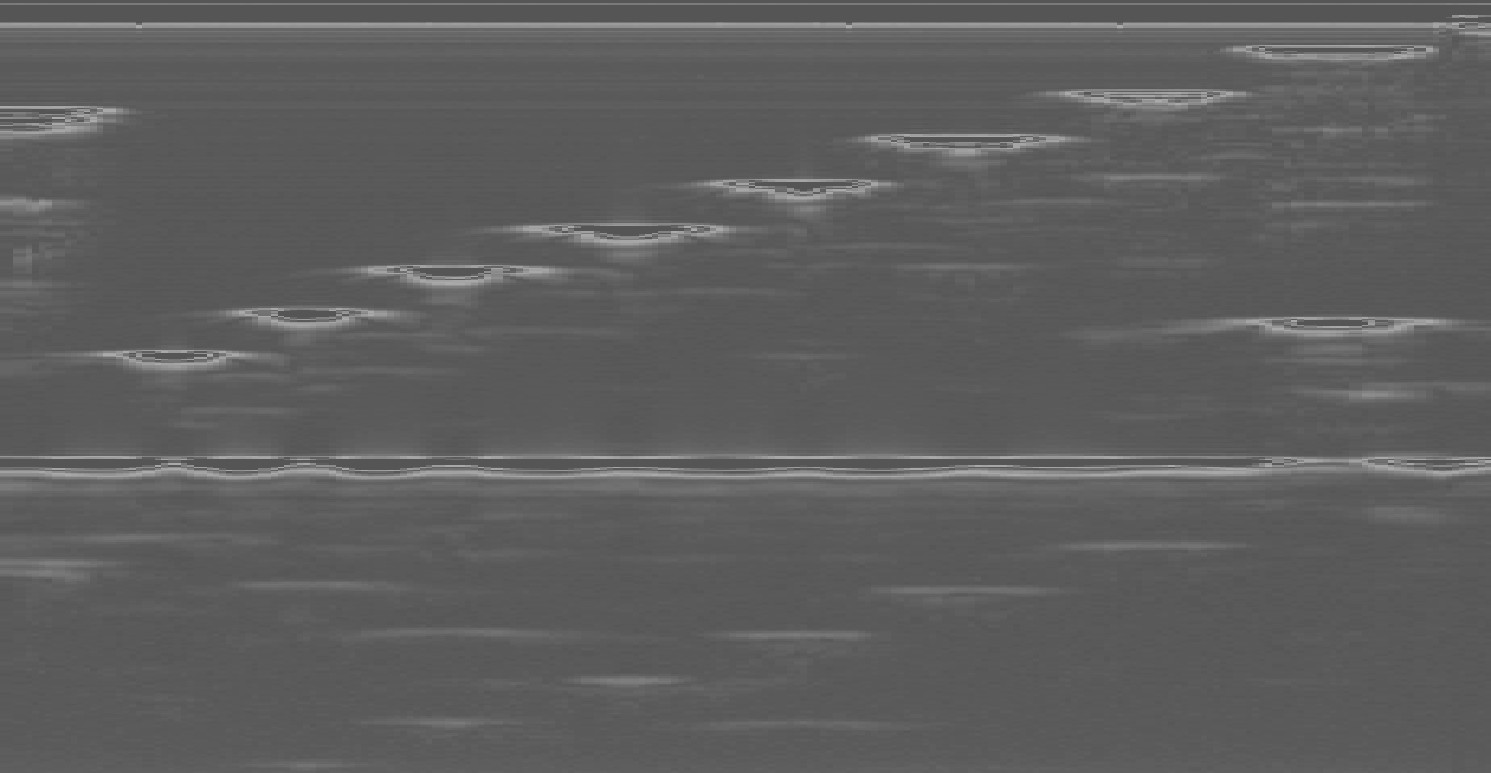
\includegraphics[width=0.8\linewidth]{data/US1_daten/b_scan_oben.jpg}
    \captionsetup{width=0.765\linewidth}
	\caption{Abbildung des Acrylblocks mit B-Scan von oben.}
	\label{fig:oben}
\end{figure}
\begin{figure}[H]
    \centering
	
\includegraphics[width=0.8\linewidth]{data/US1_daten/b_scan_u.jpg}
    \captionsetup{width=0.765\linewidth}
	\caption{Abbildung des Acrylblocks mit B-Scan von unten.}
	\label{fig:unten}
\end{figure}

Die Messwerte des B-Scan sind in der \autoref{tab:bscan} aufgetragen. Für $k =10$ konnte kein Wert
%%%%%
$a_k$
%%%%%
aufgenommen werden, daher wird dieser im Folgenden ignoriert.
\begin{table}[H]
    \centering
    \caption{Messwerte des B-Scan.}
%%%%%
	\input{build/tab_2.tex}
%%%%%
    \label{tab:bscan}
% \begin{tabular}{c c c}
% \toprule
% Loch & $\text{Laufzeit } t / \si{\micro\second} $& $ d/ \si{mm}$\\
% \midrule
%  3 & 15.1 & 63.3 \\
%  4 & 23.6 & 55.8 \\
%  5 & 32.4 & 48.2 \\
%  6 & 40.8 & 40.8 \\
%  7 & 48.9 & 33.0 \\
%  8 & 56.5 & 24.8 \\
%  9 & 64.7 & 16.8 \\
% 10 & - &  9.0 \\
% 11 & 17.2 & 57.4 \\
% \bottomrule
% \end{tabular}
\end{table}

%%%%%
Analog zu den Daten in Tabelle~\ref{tab:ascan} lassen sich aus den Verhältnissen in Tabelle~\ref{tab:bscan} die Mittelwerte $\num{1.070}$
für $a_k \, / \, a'_k$ und $\num{1.069}$ für $b_k \, / \, b'_k$ nach Vorschrift~\eqref{eqn:mittelwert} berechnen. Gleiches Vorgehen wie
zuvor liefert dann die prozentualen Abweichungen
\begin{align*}
	\increment a_k &= a_k \, / \, a'_k - 1 = \qty{7.0}{\percent} \\
	\increment b_k &= b_k \, / \, b'_k - 1 = \qty{6.9}{\percent} \: .
\end{align*}
%%%%%
% Für die prozentuale Abweichung erhält man als Mittel
% \begin{align*}
% \bar{\increment a_k} &= 1.2 \% \\
% \bar{\increment b_k} &= 4.5 \%.
% \end{align*}


\subsection{Untersuchung des Auflösungsvermögens} % Auslösungsverfahrens} % (fold)
\label{sec:Untersuchung des Auslösungsverfahrens}

Die Löcher $k = 1$ und $k = 2$ wurden mittels A-Scan jeweils mit einer $\SI{1}{\mega\hertz}$ Sonde und mit einer
$\SI{2}{\mega\hertz}$ näher betrachet. Die dabei aufgenommenen Messergebnisse sind in \autoref{fig:plot2} und \autoref{fig:plot3}
zu sehen.

\begin{figure}[H]
	\includegraphics{build/plot2.pdf}
	\captionsetup{width=0.765\linewidth}
	\caption{A-Scan für die Löcher $k = 1$ und $k = 2$ mit einer $\SI{1}{\mega\hertz}$ Sonde.}
	\label{fig:plot2}
\end{figure}
In der \autoref{fig:plot2} ist bei $d = \SI{20}{\milli\meter}$ nur ein breiter Peak zu sehen, anhand dessen können die beiden Löcher nicht unterschieden werden.

\begin{figure}[H]
	\includegraphics{build/plot3.pdf}
	\captionsetup{width=0.765\linewidth}
	\caption{A-Scan für die Löcher $k = 1$ und $k = 2$ mit einer $\SI{2}{\mega\hertz}$ Sonde.}
	\label{fig:plot3}
\end{figure}
An der Stelle $d = \SI{20}{\milli\meter}$ sind zwei eindeutige Peaks zu erkennen, welche den beiden Löchern $k = 1$ und $k = 2$
zugeordent werden können.
% subsection Untersuchung des Auslösungsverfahrens (end)

\subsection{Untersuchung des Brustmodells mittels B-Scan}
\label{sec:Untersuchung des Brustmodells mittels B-Scan}

Das gegebene Brustmodell wurde mittels B-Scan mehrmals untersucht, dabei waren die Messungen nicht alle gut, daher wurden 
die unbrauchbaren Bilder verworfen.

\begin{figure}[H]
    \centering
	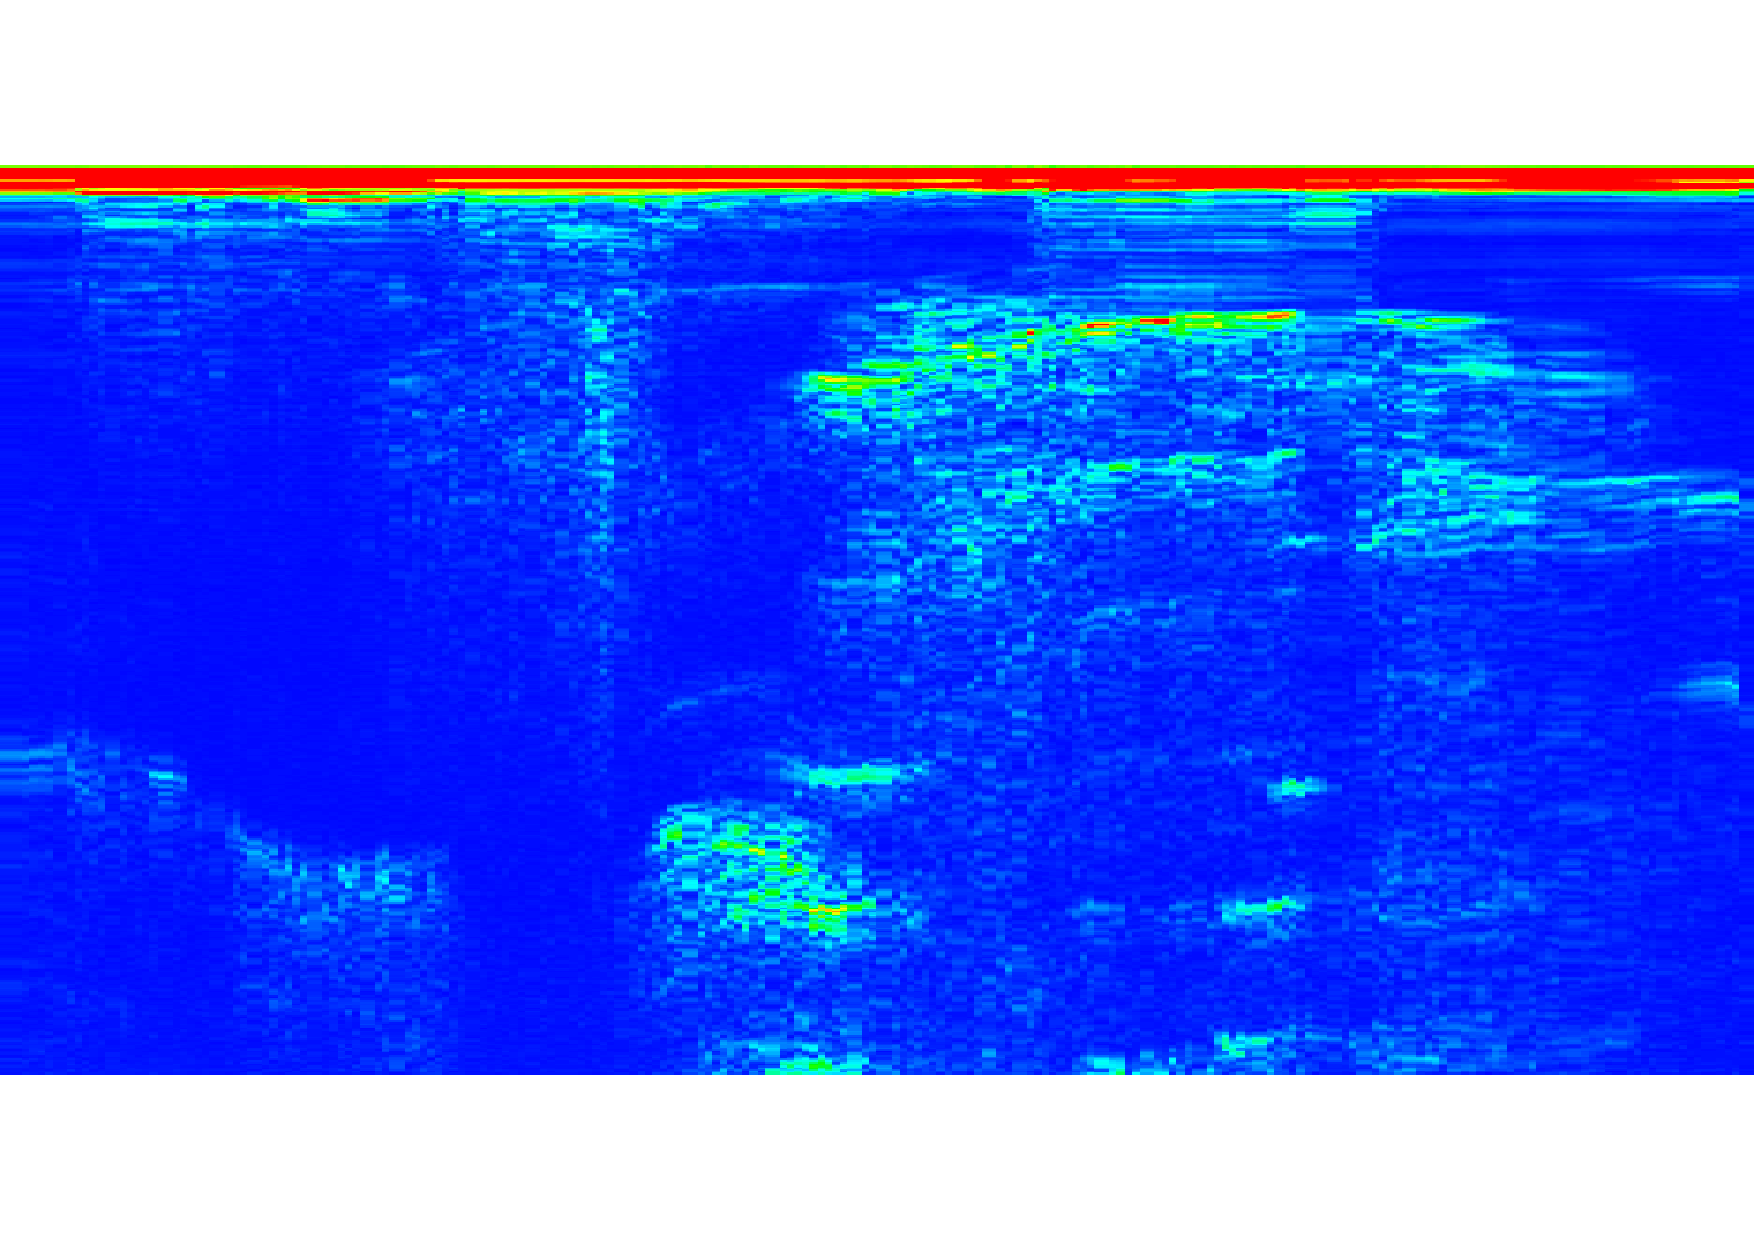
\includegraphics[width=0.8\linewidth]{content/grafik/Tumor_2.pdf}
    \captionsetup{width=0.765\linewidth}
	\caption{Erster B-Scan der Brustmodells.}
	\label{fig:b1}
\end{figure}

\begin{figure}[H]
    \centering
	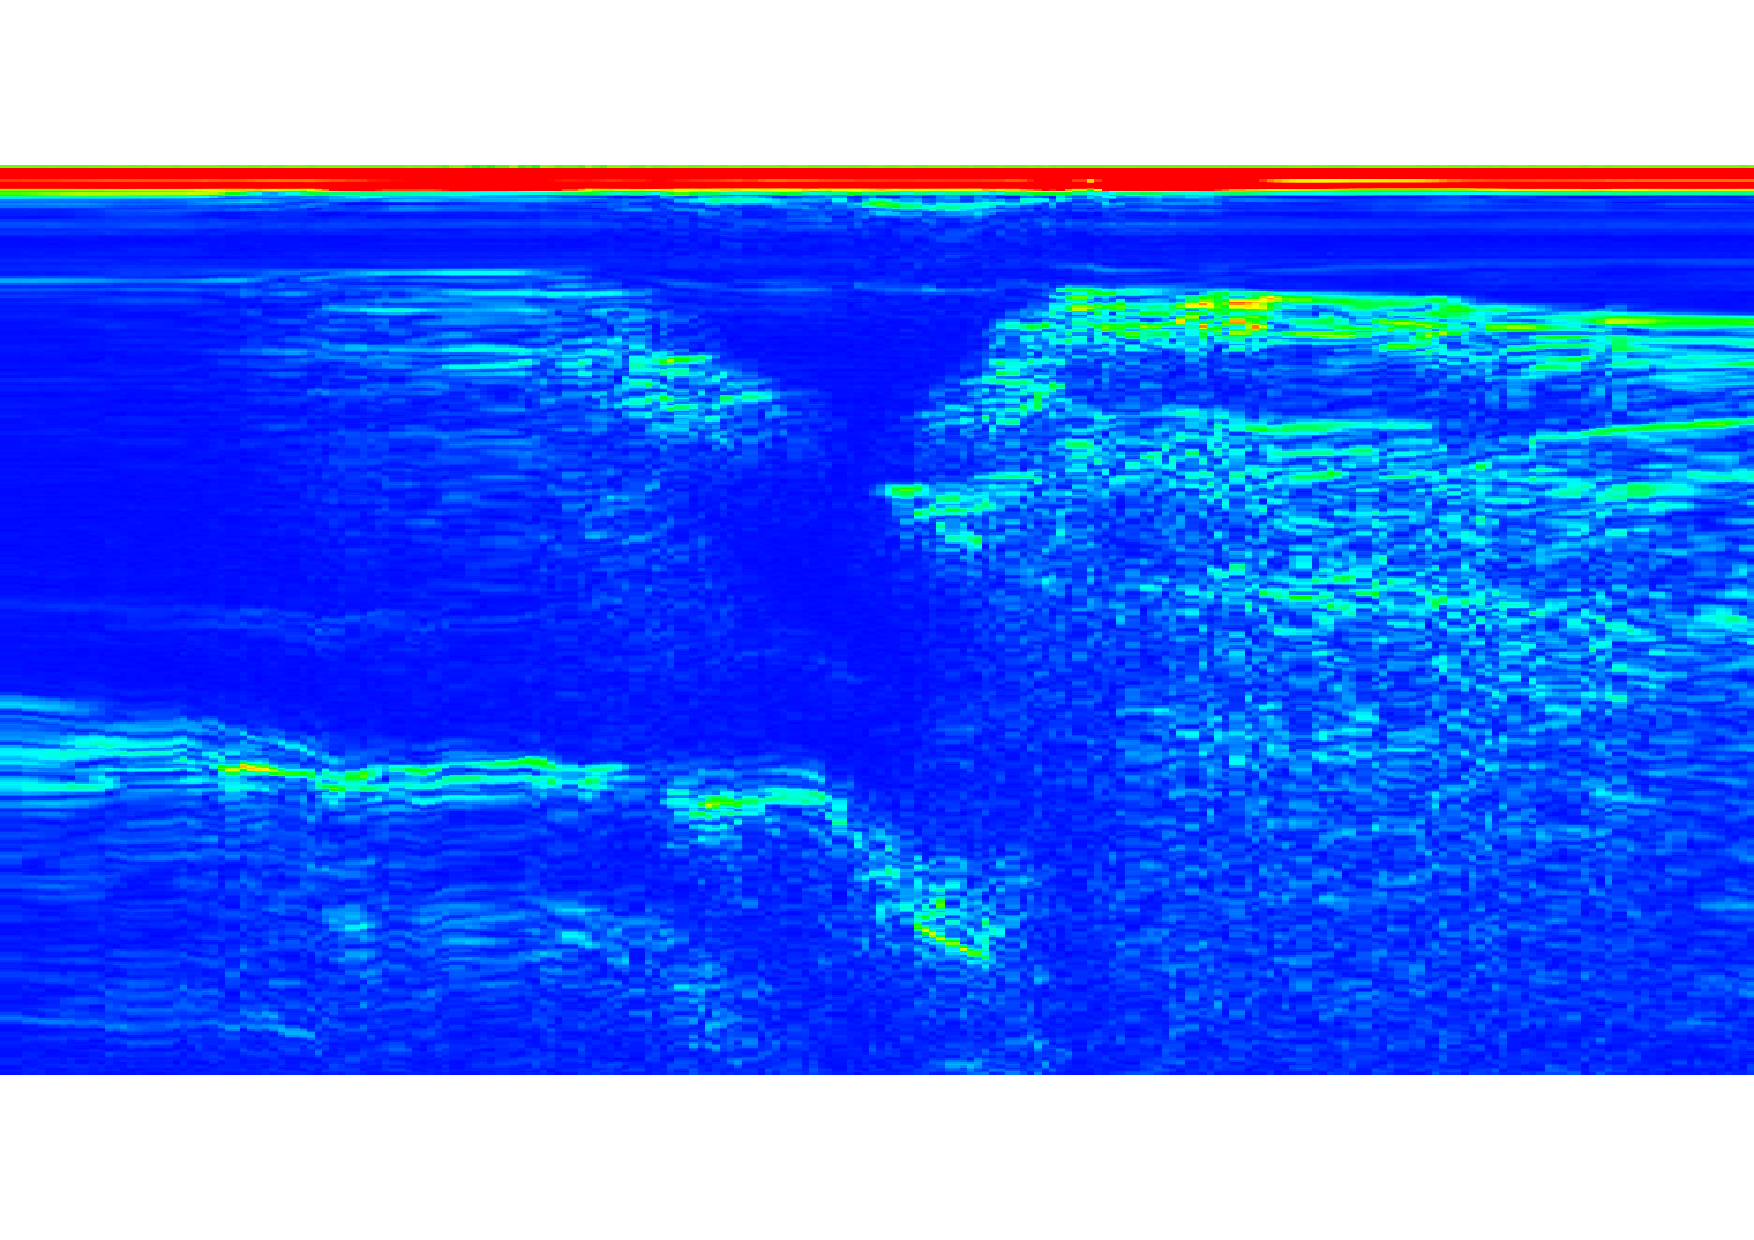
\includegraphics[width=0.8\linewidth]{content/grafik/Super_Tumor.pdf}
    \captionsetup{width=0.765\linewidth}
	\caption{Zweiter B-Scan der Brustmodells.}
	\label{fig:b2}
\end{figure}

Anhand der \autoref{fig:b2} kann gesagt werden, dass es sich bei den zwei oberen Arealen um die gesuchten
Störstellen handelt. Der rechte obere Fleck ist aufgrund der farblich gekennzeichneten höheren Dichte der Tumor.
Die rötlichen Farben entsprechen helleren Bereichen und damit höheren reflektierten Anteilen, folglich ist das Gewebe dichter.
Der linke Bereich deutet auf eine Zyste hin, da diese kein Knoten, sondern ein Hohlraum ist und auf dem Bild diffuser erscheint.

% Diskussion: Resultate mit Fehler/Genauigkeit zusammenstellen, Literaturwerte/Messmethoden/Ursachen vergleichen
% Literatur: Verwendete Literatur/Grafiken/Werte/Programme
% Anhang: Kopie der analog eingetragenen Messdaten
\section{Diskussion}
\label{sec:diskussion}

Beim Vergleich der theorethischen Kennlinie des Geiger-Müller Zählrohrs (\autoref{fig:diagramm}) und der gemessenen Kennlinie
fällt auf, dass sich der Verlauf der experimentellen Kennlinie der theorethischen vom Verlauf annähert.
Die Plateau-Länge von $\SI{340}{\volt}$ und die lineare Plateau-Steigung von $ s= \qty{0.018(3)}{\per\volt}$ passen ebenfalls
zu den erwarteten Werte für das Zählrohr. Der Verlauf der detektierten Teilchen in Abhängigkeit zur Spannung 
weist einen ähnlichen Verlauf auf wie die gemessene Kennlinie des Geiger-Müller Zählrohrs.
Bei der Spannungsquelle des Geiger-Müller Zählrohrs ist in der Anleitung angegeben, dass diese eine halbe Stunde
vor Versuchs Anfang angestellt werden sollte. Bei der Durchführung des Versuches wurde dieser Zeitraum um ungefähr 15 Minuten 
gekürzt. Dies kann die Abweichungen erklären.

Für die Bestimmung der detektierten Teilchen wurde für den Strom $I$ ein Fehler von $0.05 \si{\micro\second}$ angenommen.
Bei der berechnung der detektierten Ladungsträger war dieser Fehler irrelevant , da er in einer zu kleinen Größenordnung ist und 
damit für die Rechnung kein Rolle spielt.

Die Totzeit $\tau$ wurde über zwei Verfahren bestimmt. Beim Ablesen am Osziloskop wurde für $\tau$ ein Wert von
$\left(150 \pm  10\right) \si{\micro\second}$ bestimmt. Über die Zwei-Quellen-Methode wurde ein Wert von $\tau =\left(2.03 \pm 0.07\right) \si{\micro\second}$
berechnet. Die Werte befinden sich nicht in einer Größenordnung und weichen daher zu stark von einander ab, als das dies annehmbar ist.
Diese große Abweichung lässt sich durch einen Fehler des Zählrohrs erklären. Während der Messung der Zählraten der Proben
hat die Messung bei 67233 staatt 99999 abgebrochen. Die genau Ursache dieses Fehlers konnte nicht bestimmt werden.

\newpage

\newpage
\printbibliography{}
\nocite{matplotlib}
\nocite{numpy}
\nocite{scipy}
\nocite{uncertainties}
\nocite{reback2020pandas}

\newpage
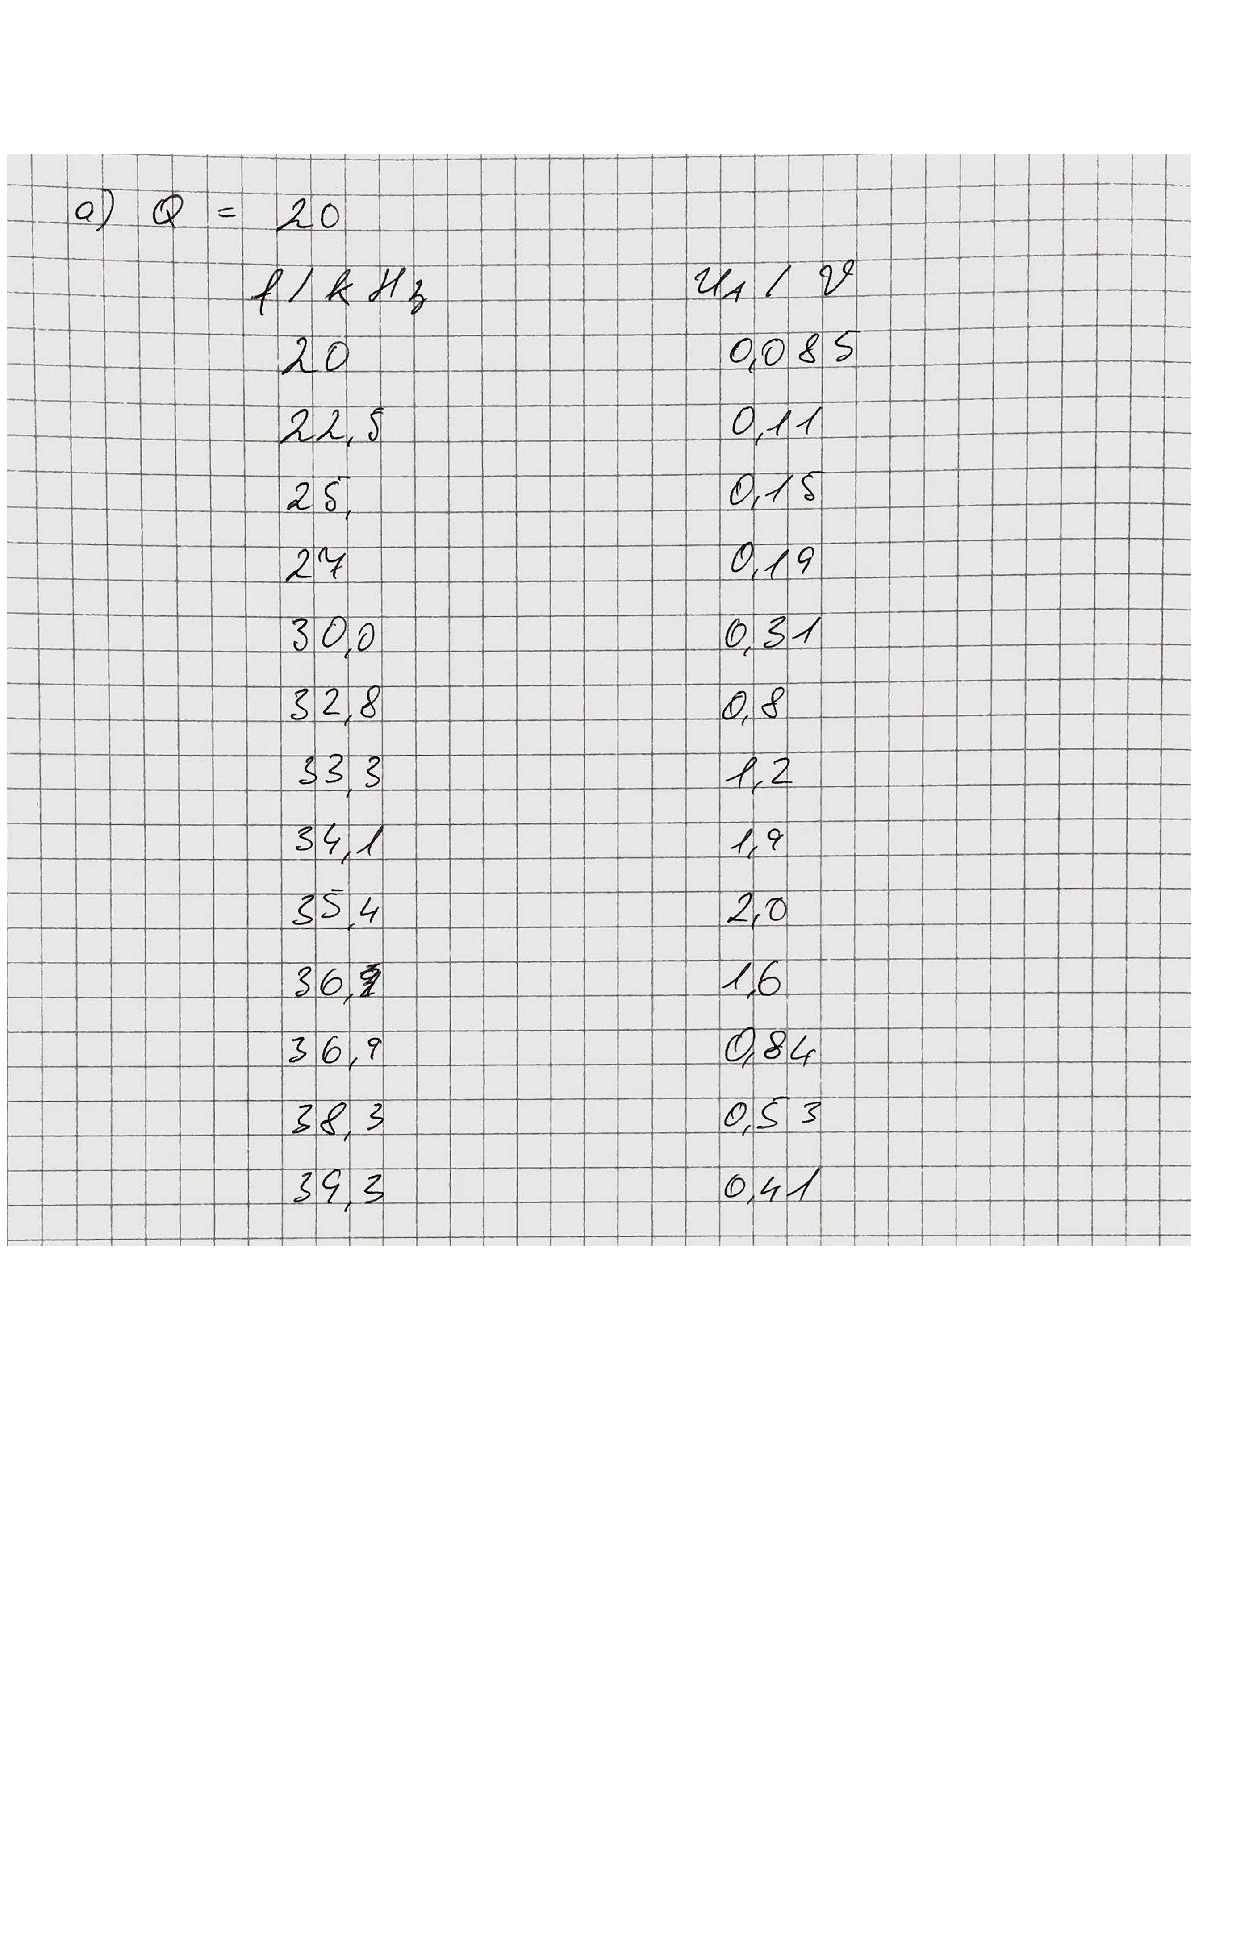
\includepdf[pages=-]{tables/messdaten.pdf}

\end{document}
